

%\documentclass[conference]{IEEEtran}
%\IEEEoverridecommandlockouts
\documentclass{article}  
\twocolumn

\usepackage{graphicx}
\usepackage{algorithm}
\usepackage{algorithmic}
\usepackage{amsmath}
\usepackage{adjustbox}
\usepackage{authblk}
\usepackage{pbox}
\usepackage{float}
\usepackage[margin=1in]{geometry}
\author[1]{Dalia Ibrahim}
\author[2]{Carlos Dasaed Salcedo}


{
    \makeatletter
    \renewcommand\AB@affilsepx{: \protect\Affilfont}
    \makeatother
        
        

    \affil[ ]{Studnet ID}

    \makeatletter
    \renewcommand\AB@affilsepx{, \protect\Affilfont}
    \makeatother

    \affil[1]{201893217}
    \affil[2]{201892008}
    
        \makeatletter
\setlength{\floatsep}{5pt}
\setlength{\textfloatsep}{5pt}
    \makeatother
    
}

\begin{document}  

\title{ Assignment 2: Choosing the Best Parameters to Use for a Binary KNN classifier using on 5-fold cross-validation}


\maketitle
 \section{Introduction}
For this assignment, we have implemented a cross-fold validation algorithm from scratch using Python and the following libraries: pandas, numpy, math, random, and sys. To improve the efficiency of the algorithm, unsupervised filtering was also used based on the calculations of a correlation matrix and variances of the data using sklearn libraries. The other sklearn libraries included in the final program were used to calculate KNN and related precision metrics. To run the program, the following line must be executed from the command line in Linux: \\
\$python3 A2\_t2.py [DataFile.tsv]

 \section{ Feature Selection}
To improve the performance of the algorithm, a process of feature selection was applied by eliminating least relevant features in the model. Eliminating features reduces the amount of calculations and overall complexity of the algorithm, but doing so cannot be done in a trivial and random manner. The process by which the features were eliminated will be described in the following subsections. 

\subsection{Selecting Highly Correlated Features}


The correlation matrix function in the sklearn libraries was used to find highly correlated features. Since highly correlated features bring the same information, some of these can be removed without significantly affecting the overall performance. For this particular data set, various thresholds were tested, but 0.80 was determined to be the ideal candidate, as it reduced the features from 348 to 305, without affecting the performance.
 
\subsection{Removing low-variance features}

The next method of feature selection consisted in the removal of features with low variance across all the observations. For example, if a feature has zero variance, it means that all its values are the same, and therefore does not add any new information to the model. In our algorithm, a threshold of 0.9 was selected to allow for a total of up to 5 features. 

 \section{Main Pseudo-code}
This section only includes the cross validation function, since it was the main purpose of the assignment. The fold splitter function divided the data into 5 folds with similar proportions of 0s to 1s as in the original data set. As the cross validation function iterates through the folds generated from the fold splitter, the SplitData function converts the fold in the current iteration into the testing data, and merges all the other folds into the training data. These functions were manually programmed as they are not part of the sklearn libraries used, and their respective pseudo-code can be found in the appendix section of this PDF if interseted. 


 \subsection{Cross Validation}
 
 Algorithm 3   in Lecture notes is implemented.
And the result grid stores the average  AUC values of features space against all possible KNN values.
After the cross-correlation loop, the three corrosponding models of highest  AUC are chosen to be the best models. However, the two correosponding models of lowest Auc is chosen to be the worst model.



\section{Loss Function }  
The Area Under the Curve (AUC) was chosen as the loss function. The best model was selected based on the ROC graph with the highest AUC, while the one with the smallest AUC was selected as the worst.

\section{Deciding on Performance}  
Since there are several different performance metrics that can be used to determine how good an algorithm will perform, it is important to make an effort to chose an adequate performance metric for the task at hand. Upon inspection of the training data, it became obvious that the amount of zeros drastically outnumbered the amount of ones by ratio of about 10 to 1. This meant that blindly using accuracy as the factor to determine the best model would be insufficient, since an algorithm that always predicts the output class to be zero would actually be correct 90\% of the time. Therefore, to determine which model was best, we decided to focus on identifying instances of class 1. In other words, we considered ones as positives, and zeros as negatives for the TPR, FPR, ROC curves, loss function and selection of our best model.

 \section{Results}
To better display the results of our algorithm, we used the sklearn metrics library, which allowed us to generate Figures 1 and 2. Figure 1 shows a graphical representation of the best and worst models with the current algorithm. Since 25 neighbors yielded the best results in our algorithm, we decided to run a classical implementation of KNN without any filtration of the features. Our best model outperform the classical model with all features. The AUC of proposed model was 0.88 with K = 25  using four features and  the AUC of  Classical model with 348 features  was 0.86 when K= 23.

  Even though the time of execution was not a parameter to consider for the assignment and was not officially recorded, we can say with certainty that our algorithm ran a lot faster since it had a lot less parameters to take into consideration for the KNN. 

 \begin{table}[H]
\begin{tabular}{|l|l|l|l|}
\hline
           & \multicolumn{3}{l|}{\textbf{K= 23, NumOfFeatures=4, AUC = 0.87}}                                                    
            \\ \hline  
           & \multicolumn{3}{l|}{\textbf{ TP=679 , TN=15 , FP=45 , FN=25  }}                                                    
            \\ \hline  
            
           & \multicolumn{1}{c|}{\textbf{Precision}} & \multicolumn{1}{c|}{\textbf{Recall}} & \multicolumn{1}{c|}{\textbf{F1-Score}} \\ \hline
\textbf{0} & 0.94 & 0.98                                 & 0.96                                   \\ \hline
\textbf{1} & 0.62 & 0.36                                 & 0.45 \\ \hline
\end{tabular}
\caption{Performance metrics of the best model}
\end{table}

\begin{center}
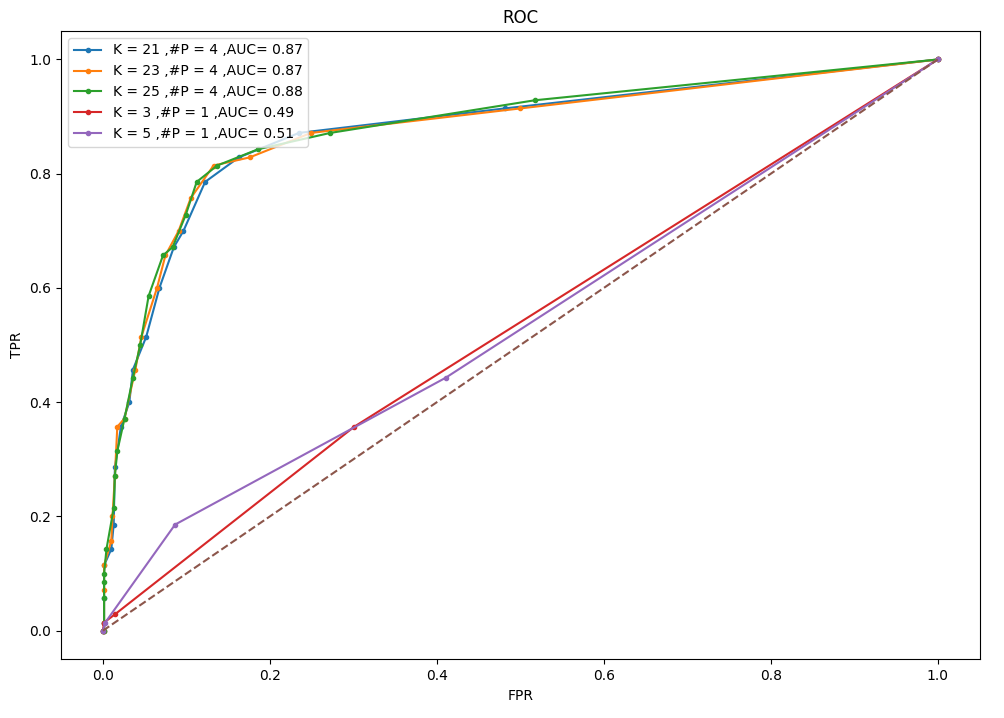
\includegraphics[scale=.2]{ROCNew.png} %{Roc2.png} 
\end{center}
Fig. 1 ROC Curve for the 3 best models and the 2 worst models\\

\begin{center}
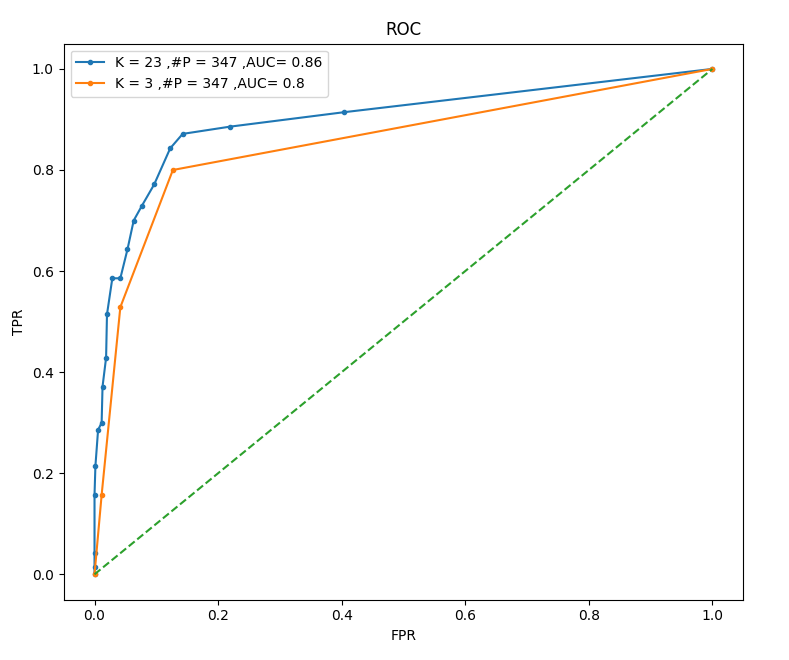
\includegraphics[scale=.25]{ROC_allfeatures.png}
\end{center}
Fig. 2 ROC for KNN with 3 and 23 neighbors, and all the features in the dataset.


\section{Conclusion}
KNN is a powerful and useful machine learning classifier. However, just like any other classifier, without the proper parameters such as an adequate feature selection, number of neighbors, and correct training set, the model can easily become skewed or flawed. For this reason, it is important to select the proper performance metrics and to run cross validation tests with at least 5 folds. In our particular case, using 5 fold cross validation, and selecting the features based on a correlation matrix and variance, consistent models with AUCs of up to 0.88 were obtained.   \\ 

\section{Appendix}
\subsection{FoldSplitter()}

\begin{algorithm}[H]
\caption{Split Data in K folds}
\begin{algorithmic}[1]
\REQUIRE kfolds  \COMMENT{kfolds = 5 was used}
\STATE $ data \gets dataframe(DataFile.tsv)$
\STATE $ class0 \gets $ data.where(class=0).ShuffleRows() 
\STATE $ class0partition \gets  Rows In class0 / kfolds $
\STATE $ class1 \gets $ data.where(class=1).ShuffleRows()
\STATE $ class1partition \gets  Rows In class1 / kfolds $
\STATE $ leftOvers0 \gets $class0 rows after(class0partition * cvfolds)]
\STATE $ leftOvers1 \gets $class1 rows after(class1partition * cvfolds)]
\STATE $ leftOvers \gets $ concatenation( leftOvers0, leftOvers1)
\STATE $ theFolds \gets newPythonDictionary$
	\FOR { i=0 \textbf{to} kfolds-1 }
        \STATE  $create fold\textbf{i} $ \COMMENT{i = corresponding iteration in the for cycle} 
      	\STATE $class0Range \gets $class0[\textbf{from} i * class0partition \textbf{to} (i * class0partition)+class0partition  
      	\STATE $class1Range \gets$ class1[\textbf{from} i * class1partition \textbf{to} (i * class1partition)+class1partition   
      	\STATE $fold\textbf{i} \gets class0range + class1range  $
		\IF{$i = kfolds-1 $}
	  	\STATE $fold\textbf{i} \gets fold\textbf{i} + leftOvers $ 
		\ENDIF	
    \STATE $theFolds[fold\textbf{i}] = TempData $  	
	\ENDFOR
\STATE return theFolds 
\end{algorithmic}
\end{algorithm}

 \subsection{SplitData()}
\begin{algorithm}[H]
\caption{Create Learning and Training Data}
\begin{algorithmic}[1]
\REQUIRE DictionaryOfFolds , iterNum 
\STATE $ testFold \gets fold\{iterNum\}$ \COMMENT{iterNum refers to the iteration number, such that testFold will get fold1,fold2,...,fold5}
\STATE $testDF \gets DataFrame(testFold) $
\STATE $trainDF \gets NewDataFrame $
	\FOR { foldKey, foldValue \textbf{in} DictionaryOfFolds } 
		\IF{$foldkey = testFold $}
		  	\STATE Skip this Iteration 
		\ENDIF
        \STATE $trainDF.append(foldValue)$
  	\ENDFOR
\STATE $xtraining \gets $ trainDF without the last column 
\STATE $ytraining \gets $ testDF without the last column
\STATE $xtesting \gets $ trainDF with only the last column
\STATE $ytesting \gets $ testDF with only the last column
\STATE return xtraining, xtesting, ytraining, ytesting

\end{algorithmic}
\end{algorithm}


\end{document}
